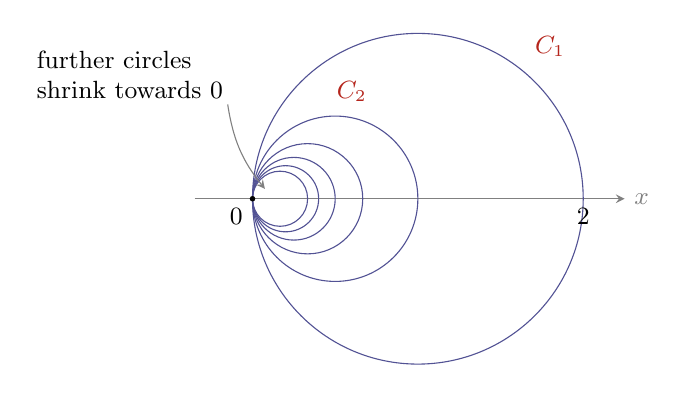
\begin{tikzpicture}[x=2.1cm,y=2.1cm,font=\small,>=stealth]
\draw[gray,->] (-.35,0)--(2.25,0) node[right] {$x$};
\foreach \n in {1,2,3,4,5,6} {
\draw[MidnightBlue!75] ({1/\n},0) circle[radius={1/\n}];}
\fill (0,0) circle (1pt);
\node[below left] at (0,0) {$0$};
\node[below] at (2,0) {$2$};
\node[above right,BrickRed] at (1.65,.8) {$C_1$};
\node[above,BrickRed] at (.6,.53) {$C_2$};
\node[align=left,anchor=east] at (-.12,.75) {further circles\\shrink towards $0$};
\draw[->,gray] (-.15,.57) to[bend right=15] (.075,.06);
\end{tikzpicture}
